\documentclass[A4paper, 11pt]{book}
\usepackage{atm_config}

\title{Appunti del corso di 
	\\ \Huge Fisica dell'Atmosfera}
\author{A cura di Lorenzo Uboldi}
\makeindex
\begin{document}
\frontmatter
\maketitle

	
% Colophon
\null % Bisogna inserire qualcosa prima di \vfill, altrimenti non funziona
\vfill % Riempie lo spazio verticale della pagina
\hspace*{-1.5em}\includegraphics[scale=.7]{figures/by-sa.eps}
\begin{flushleft}
	Quest'opera è stata rilasciata con licenza \emph{Creative Commons} Attribuzione - Condividi allo stesso modo 4.0 Internazionale. Per leggere una copia della licenza visita il sito web \url{https://creativecommons.org/licenses/by-sa/4.0/}.\\[1cm]
	Versione aggiornata al \today,\\
	Lorenzo Uboldi (\href{mailto:lorenzo.uboldi@studenti.unimi.it}{\ttfamily lorenzo.uboldi@studenti.unimi.it}), Milano.\\[0.2cm]
	L'ultima versione, aggiornata e rivista, è sempre disponibile a: \url{https://github.com/ulorentz/FisicaAtmosfera}
	
\end{flushleft}

\cleardoublepage

\tableofcontents
\mainmatter
\chapter{Pressione}
L'evidenza della pressione atmosferica può essere mostrata, ad esempio, con un barometro di Torricelli: capovolgendo un tubo con una sola apertura pieno di mercurio in una bacinella con lo stesso liquido, il livello del mercurio scende fino ad assestarsi ad una determinata altezza. La pressione atmosferica esercita una forza sul liquido nella bacinella che si oppone al peso che farebbe scendere il mercurio nel tubo. Precisamente, se $P_{B}$ è la pressione sulla bacinella e $P_{A}$ è quella esercitata dal mercurio nel tubo, $S$ è la sezione del tubo e $h_{\ch{Hg}}$ l'altezza della colonna di mercurio, all'equilibrio idrostatico si ha:
\begin{equation}
	P_{B}=P_{atm}=P_{A}=\frac{m_{\ch{Hg}}g}{S}=\frac{\rho_{\ch{Hg}} S h_{\ch{Hg}} g}{s}=\rho_{\ch{Hg}} h_{\ch{Hg}} g 
\end{equation}
il mercurio si assesta ad un'altezza di 76 cm, che corrispondono alla pressione media atmosferica di 1013 hPa.
\section{Origine della pressione atmosferica}
Supponiamo di avere un'atmosfera composta da un'unica particella di massa $m$ ad altezza $h$ rispetto alla superficie terrestre; inizialmente ferma, essa cade e subisce un urto elastico. La legge oraria è
\begin{equation}
	y(t)=h-\frac{1}{2}gt^2
\end{equation}
mentre la velocità finale all'impatto impatto della particella è
\begin{equation}
	v_f=\sqrt{2gh}.
\end{equation} 

Detto $\hat{j}$ il versore ortogonale uscente dalla superficie terrestre, la variazione di velocità è
\begin{align}
	\Delta \vec{v}=2\sqrt{2gh}\hat{j}
\end{align}
per cui, dato che il tempo che la particella impiega a cadere e tornare alla posizione iniziale è $t=2\sqrt{2h/g}$, la forza media che riceve è:
\begin{equation}
	\langle\vec{F}\rangle=\frac{m\Delta\vec{v}}{t}=\frac{2m\sqrt{2gh}\hat{j}}{2\sqrt{2h/g}}=mg\hat{j}.
\end{equation}

Per il terzo principio della dinamica, la forza media che riceve il pianeta è l'opposto, ovvero $\langle\vec{F}\rangle=-mg\hat{j}$. Nel caso di molte molecole, invece della massa della singola particella, si ha:
\begin{equation}
	\vec{F}=-M_{atm}g\hat{j}
\end{equation}
dove $M_{atm}\simeq 5.26 \cdot 10^{18}$kg.

L'origine della pressione atmosferica, dunque, è dovuta all'attrazione gravitazionale sulle molecole d'aria. 
\section{Equilibrio idrostatico in atmosfera}
Dal momento che l'atmosfera è estesa, essa interagisce con sè stessa: gli strati superiori comprimono quelli inferiori. La pressione, pertanto, varia lungo la coordinata zeta. 

Consideriamo una colonna di atmosfera come in figura (INSERIRE), se lo strato di aria compreso tra il punto A e B, la cui superficie di base è $S$, si trova in equilibrio dinamico, allora vale che $\sum\vec{F}=0$. Supponendo che la pressione sia costante lungo le coordinate $x$ e $y$, ovvero che $P=P(z)$, si ha la condizione\footnote{Nota che la pressione subita da un elemento di fluido è sempre diretta verso l'interno}
\begin{equation}\label{eq1}
	(\sum\vec{F})_z=P_A S - P_B S -mg =0.
\end{equation}

Considerata una variazione infinitesima lungo $z$, la pressione in B è 
\begin{equation}
	P_B=P_A+\frac{\partial P}{\partial z}dz
\end{equation}
e l'equazione \eqref{eq1} diviene
\begin{align}
	&P_A S - P_A S -\frac{\partial P}{\partial z}dzS -\rho S g dz=0\\
	&\Rightarrow -\frac{\partial P}{\partial z}-\rho g =0.
\end{align}
Se $P=P(z)$ (ovvero non dipende dalle componenti $x$ e $y$) si ha l'\emph{equazione di equilibrio idrostatico}:
\begin{equation}\label{idro}
	dP=-\rho g dz.
\end{equation}

In tre dimensioni, la forza dovuta alla pressione che subisce un elemento di atmosfera è\footnote{in fisica dell'atmosfera conviene ragionare in termini di unità di massa, in modo da eliminare la dipendenza da quest'ultima.}
\begin{equation}
	\frac{\vec{F}_P}{m}=-\frac{1}{\rho}\left(\frac{\partial P}{\partial x},\frac{\partial P}{\partial y}, \frac{\partial P}{\partial z}\right)
\end{equation}
ovvero
\begin{equation}
	\frac{\vec{F}_P}{m}=-\frac{1}{\rho}\nabla P.
\end{equation}

L'atmosfera organizza l'evoluzione della pressione ($\nabla P$) al fine di contrastare la forza gravitazionale, è da notare che $\frac{\partial P}{\partial z}$ è ordini di grandezza più grande delle altre componenti; inoltre, lungo la coordinata $z$, la pressione deve necessariamente decrescere affinché vi sia equilibrio. 

\section{Variazione della pressione lungo la coordinata $z$}
Dividendo ambo i lati dell'equazione dei gas perfetti per la massa, si ottiene:
\begin{equation}\label{gas}
	\frac{PV}{m}=\frac{n RT}{m} \rightarrow \frac{P}{\rho}=\frac{R}{M}T
\end{equation}
dove $M$ è la massa molare. Si noti che l'equazione dei gas perfetti è accurata quando si è lontani dai cambiamenti di stato, per le maggiori componenti dell'atmosfera (\ch{O_2} e \ch{NO_2}) questo è sicuramente vero. 

Inserendo la \eqref{gas} nell'equazione dell'equilibrio idrostatico \eqref{idro}, si ottiene:

\begin{equation}\label{dp}
	dP=-\frac{PM}{RT}g dz,
\end{equation}
dove $M$ è la massa molare. Considerati i maggiori componenti atmosferici, ovvero 75\% di azoto ($M_{N_2}=28$g/mol) e circa 25\% di ossigeno ($M_{O_2}=32$g/mol), si ottiene una media ponderata di $M=29$g/mol$=2.9\cdot10^{-2}$kg/mol.

Per ottenere l'andamento della pressione al variare della coordinata $z$, è necessario risolvere l'equazione differenziale \eqref{dp}. Il problema è che, in atmosfera, la temperatura è a sua volta dipendente della quota, ovvero $T=T(z)$, e, a priori, non è una funzione nota.\\


\subsection{Ipotesi di atmosfera isoterma}
L'andamento della temperatura in funzione della quota è, grossolanamente, rappresentato in figura (INSERIRE). Una tecnica per risolvere la \eqref{dp} è di considerare una temperatura media $\bar{T}$ dell'atmosfera, ad esempio di 250K, e di supporla, quindi, isoterma. 

Integrando la \eqref{dp}, si ottiene: 
\begin{align}
	\int_{P_0}^{P}\frac{dP'}{P'}&=-\int_{0}^{z}\frac{Mg}{R\bar{T}}dz'\\
	\ln P \Big|_{P_0}^P&=-\frac{Mg}{R\bar{T}}z\Big|_0^z\\
	P&=P_0\exp\left(-\frac{Mg}{R\bar{T}}z\right) \label{pz}.
\end{align}

Dalla \eqref{pz}, si intuisce che a temperature maggiori la pressione varia più lentamente all'aumentare della quota rispetto a temperature inferiori, e viceversa. Difatti, maggiore è la temperatura minore è il coefficiente che moltiplica $z$ nell'esponenziale.\\ %TODO inserire figura?

Un utilizzo della formula \eqref{pz} è per riportare le pressioni al livello del mare. Ogni stazione meteorologica è situata ad una specifica quota e per confrontare i valori di pressione rilevati in diverse coordinate geografiche è necessario confrontare dati alla stessa $z$. In altre parole per studiare $\frac{\partial P}{\partial x}$ e $\frac{\partial P}{\partial y}$ è necessario che $z$ sia costante.

Ad esempio, si supponga di effettuare una rilevazione a Linate (la cui altitudine è $z=104$m) di $P=1006.4$hPa ad una $T=10^\degree$C. Per calcolare la pressione al livello del mare:

\begin{equation*}
	P(-104\text{m})=1006.4\text{hPa}\cdot\exp\left(\frac{-29\cdot10^{-3}\text{kg/mol}\cdot 9.81\text{m/s}^2\cdot (-104\text{m})}{8.314\text{J/(mol K)} \cdot293.5 \text{K}}\right)=1019.1\text{hPa}
\end{equation*}
Da notare che la temperatura utilizzata è quella alla quota media tra l'altitudine della stazione e il livello del mare, e dal momento che nei primi strati di atmosfera il gradiente termico è di circa $0.65$K ogni 100m, si ha: $T_{media}=(283.15+0.65/2)\text{K}\sim 283.5$K.

Si deduce che, nello strato inferiore dell'atmosfera, il gradiente di pressione è di circa 12hPa ogni 100m, o anche 8 metri ogni hPa.\\

La \eqref{dp} può essere integrata per ricavare la dipendenza dalla quota dalla pressione, in situazioni come gli \emph{atmospheric soundings}\footnote{Sono dei palloni aerostatici pieni di elio che vengono lasciati liberi al fine di misurare i parametri atmosferici, ad esempio la pressione e temperatura.}, la variabile indipendente è proprio la pressione e non la coordinata $z$:
\begin{equation}
	\int_{z_1}^{z_2}dz=-\frac{RT}{Mg}\int_{P_1}^{P_2}\frac{dP}{P},
\end{equation}
ovvero
\begin{equation}
	z_2-z_1=-\frac{RT}{Mg}\ln \frac{P_2}{P_1}.
\end{equation}

Dalla \eqref{dp} si ottiene la dipendenza della densità atmosferica dalla variazione della pressione rispetto alla quota:
\begin{equation}
\rho=-\frac{1}{g}\frac{dP}{dz}.
\end{equation}
Utilizzando la \eqref{pz} si ha
\begin{equation}
\rho=-\frac{1}{g}P_0\left(-\frac{Mg}{RT}\right)e^{-\frac{Mg}{RT}z}
\end{equation}
ovvero, ricavando dall'equazione dei gas perfetti $\rho_0=\frac{P_0 M}{RT}$:
\begin{equation}\label{roz}
\rho=\rho_0 e^{-\frac{Mg}{RT}z}.
\end{equation}

La grandezza $z_0=\frac{RT}{Mg}$ viene chiamata \emph{altezza di scala} (quota necessaria affinché la pressione e la densità si abbattano di un fattore 1/e), le equazioni \eqref{pz} e \eqref{roz} possono essere riscritte come:
\begin{align}
P&=P_0e^{-\frac{z}{z_0}}\\
\rho&=\rho_0e^{-\frac{z}{z_0}}.
\end{align}

\subsection{Ipotesi di dipendenza lineare della temperatura}
Nella troposfera la dipendenza della temperatura con la quota è sufficientemente lineare (FIGURA) da poter considerare la seguente relazione:
\begin{equation}\label{tz}
	T(z)=T_0-\gamma z
\end{equation}
dove $\gamma=6.5$K/km è detto \emph{gradiente troposferico medio}.

Utilizzando la \eqref{tz} nella \eqref{dp} ed integrando, si ha:
\begin{align}
	\int_{P_0}^{P}\frac{dP'}{P'}&=-\int_{0}^{z}\frac{Mg}{R(T_0-\gamma z')}dz'\\
	\ln P'\Big|_{P_0}^P&=-\frac{Mg}{R}\left( -\frac{1}{\gamma}\right)\int_{0}^{z}\frac{dz'}{z'-T_0/\gamma}=\frac{Mg}{R\gamma}\ln\left|z'-\frac{T_0}{\gamma}\right|^z_0\\
	\ln\frac{P}{P_0}&=\frac{Mg}{R\gamma}\ln\left(\frac{\frac{T_0}{\gamma}-z}{\frac{T_0}{\gamma}}\right)=\frac{Mg}{R\gamma}\ln\left(\frac{T(z)}{T_0}\right)\\
	P(z)&=P_0\left(\frac{T(z)}{T_0}\right)^{\frac{Mg}{R\gamma}}\\
\text{invertendo si ottiene:}\nonumber\\
	z(P)&=\frac{T_0}{\gamma}\left(1-\left(\frac{P}{P_0}\right)^{\frac{R\gamma}{Mg}}\right).\label{zp}
\end{align}\\

Anche in questo caso è possibile esplicitare la dipendenza della densità dalla quota, utilizzando la \eqref{zp} si ricava:
\begin{align}
	\rho&=-\frac{1}{g}P_0\left(\frac{Mg}{R\gamma}\right)\left(\frac{T(z)}{T_0}\right)^{\frac{Mg}{R\gamma}-1}\left(\frac{\gamma}{T_0}\right)\\
	\rho&=\rho_0\left(\frac{T(z)}{T_0}\right)^{\frac{Mg}{R\gamma}-1}\label{rho}
\end{align}
dove si è utilizzato $\rho_0=\frac{P_0M}{RT}$.

Si noti che nell'atmosfera reale il gradiente termico non è costante, l'esponente della \eqref{rho} pertanto può annullarsi: in questa situazione la densità atmosferica è costante al variare della quota. L'esponente, però, non può mai essere negativo: fisicamente la statica dei fluidi impedisce una $\frac{\partial \rho}{\partial z} >0$ (l'atmosfera non sarebbe in equilibrio). Nella condizione limite in cui l'esponente si annulla si ha che $\gamma =\frac{Mg}{R}=0.034$K/m$=3.4$K$/100$m. Questo è il limite massimo che il gradiente termico può raggiungere, e proprio perché si perde la stabilità statica è detto \emph{gradiente autoconvettivo}. 

\subsubsection{Confronto tra le due ipotesi}
È utile confrontare i risultati ottenuti con l'ipotesi di atmosfera isoterma e di gradiente troposferico medio. 

Ipotizziamo di avere uno strato con $T_0=300$K,$P_0=1000$hPa, $P_{top}=200$hPa e $\bar{T}=260$K (temperatura media, necessaria per l'ipotesi di isotermia). Ci si chiede a che quota è il top dello strato. 
\begin{table}[h]
	\centering
	\begin{tabular}{c|c}
		Isoterma & Gradiente medio \\
		$z_{top}=-\frac{R\bar{T}}{Mg}\ln\frac{P_{top}}{P_0}$ & $z_{top}=\frac{T_0}{\gamma}\left(1-\left(\frac{P}{P_0}\right)^{\frac{R\gamma}{Mg}}\right)$\\
		= 12229 m & = 12157 m
	\end{tabular}
\end{table}

La situazione sopra esposta è rappresentata in figura \ref{fig:iso_vs_grad} da cui si deduce che le due ipotesi, in troposfera, sono in buon accordo. 

\begin{figure}[h]     				\centering                                                                  
   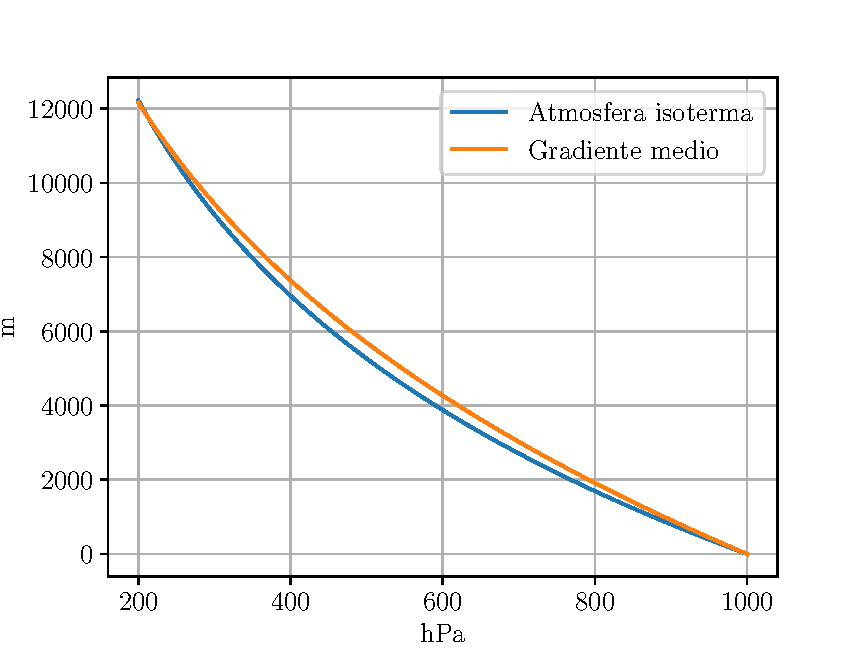
\includegraphics[width=.65\textwidth]{figures/iso_vs_grad.pdf} 
	\caption{Confronto tra atmosfera isoterma e ipotesi di gradiente troposferico medio}          
   \label{fig:iso_vs_grad}
\end{figure}         



\end{document}